\section{Analysis}
\label{sec:analysis}

The aggregate result of \S\ref{sec:experiments} hides a structurally heterogeneous picture, decomposed below along cohort, pairwise significance, stealth, perturbation-budget sensitivity, the Exact-cohort failure mode, cross-backbone replication, transfer, and anchor robustness, then consolidated under a bounded-under-stress synthesis (further replications in the released artifact).

\begin{figure*}[t]
\centering
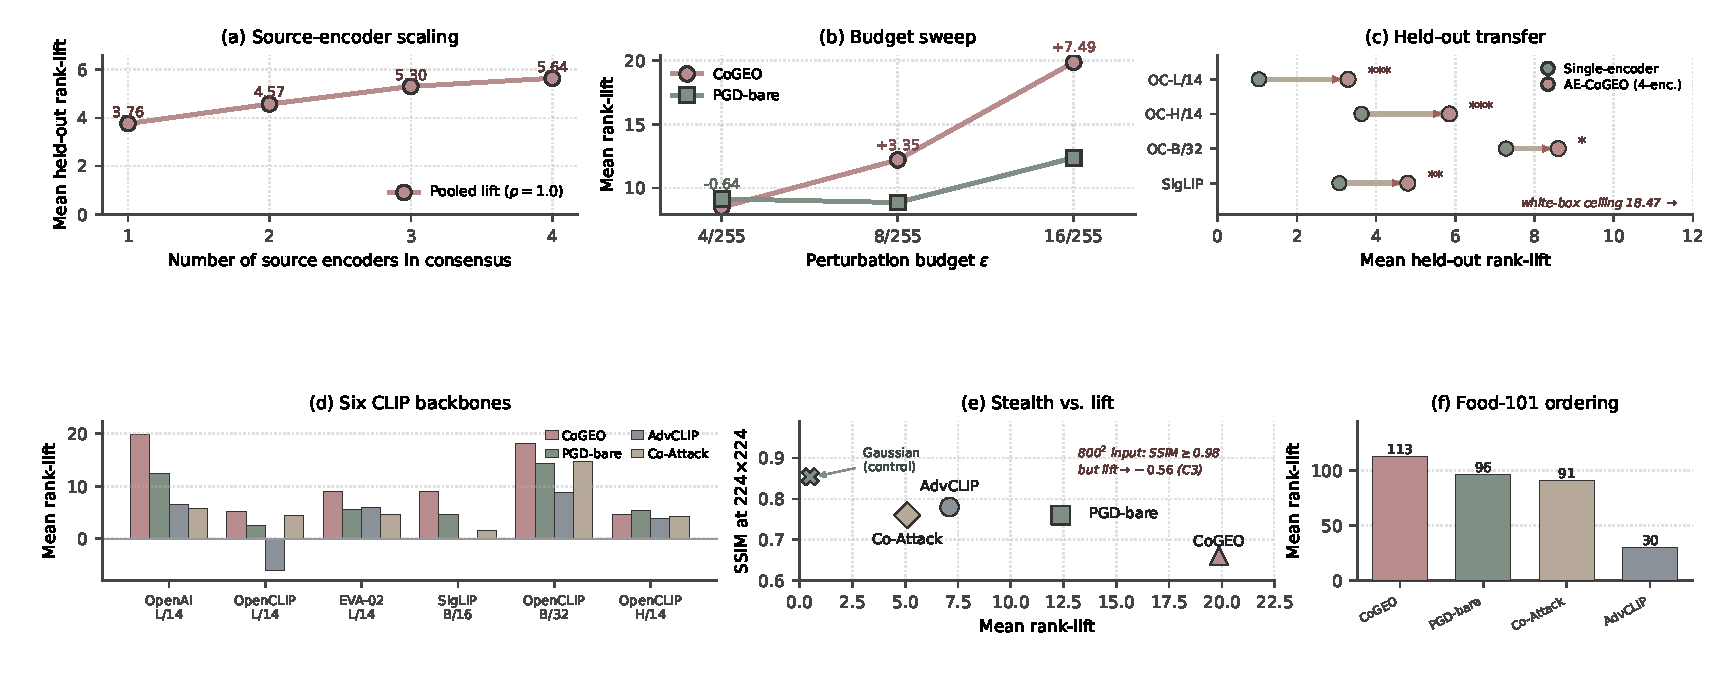
\includegraphics[width=\textwidth]{figures/fig_results_main.pdf}
\caption{AE-CoGEO transfer behavior and protocol robustness; every value matches a manuscript table. \textbf{(a)} Rank-lift scales with the source-encoder count ($3.76\to5.64$, $\rho=1.0$). \textbf{(b)} Budget sweep (OpenAI ViT-L/14): the CoGEO$-$PGD-bare margin inverts at $\eps=4/255$ ($-0.64$) and grows to $+7.49$ at $16/255$. \textbf{(c)} Held-out transfer (single-encoder~$\to$~four-encoder consensus, $n=498$, Table~\ref{tab:transfer}): the consensus lifts all four unseen encoders (one-sided paired Wilcoxon; $^{*}p<5\!\times\!10^{-2}$, $^{**}p<10^{-2}$, $^{***}p<10^{-3}$) but stays below the white-box ceiling (dashed). \textbf{(d)} Four-way rank-lift across six CLIP backbones ($\eps=16/255$): CoGEO is the unique top-1 on five of six. \textbf{(e)} Stealth/lift trade-off (Table~\ref{tab:main4way}): higher rank-lift costs SSIM, all below high fidelity at $224\times224$ (CoGEO $0.66$, AdvCLIP $0.78$). \textbf{(f)} Food-101 cross-dataset check ($505$ triples, OpenAI ViT-L/14): the ESCI ordering CoGEO $>$ PGD-bare $>$ Co-Attack $>$ AdvCLIP is preserved (gap $1.61\times\!\to\!1.17\times$).}
\label{fig:results}
\end{figure*}

\subsection{Per-cohort rank-lift decomposition}
\label{sec:analysis:cohort}

\begin{table}[t]
\centering
\caption{Per-cohort mean rank-lift over the four ESCI relevance classes ($560$-pair, OpenAI ViT-L/14, $\eps=16/255$): the per-cohort heterogeneity claim \textbf{(C2)}. Bold marks the per-cohort best; sizes $n=125$ for E/S/I and $185$ for C; values match Table~\ref{tab:main4way}.}
\label{tab:cohort}
\small
\setlength{\tabcolsep}{5pt}
\begin{tabular}{lrrrr}
\toprule
Method & Exact & Substitute & Complement & Irrelevant \\
 & ($n{=}125$) & ($n{=}125$) & ($n{=}185$) & ($n{=}125$) \\
\midrule
CoGEO     & 3.90 & 5.24 & \textbf{36.77} & \textbf{25.43} \\
PGD-bare  & \textbf{7.12} & 1.84 & 18.86 & 18.53 \\
AdvCLIP   & 1.00 & 0.94 & 14.46 & 5.53 \\
Co-Attack & 6.18 & \textbf{5.47} & $-1.86$ & 16.94 \\
\bottomrule
\end{tabular}
\end{table}

Table~\ref{tab:cohort} reports the same rank-lift quantity as Table~\ref{tab:main4way}, split across the four ESCI cohorts (sizes $n=125$ for E/S/I and $185$ for C); the split materially reshapes the headline.

Three patterns emerge. First, CoGEO's dominance is not uniform: on Exact, PGD-bare's mean exceeds CoGEO's by $\sim3.2$ positions, yet matched-pair tests find no systematic per-pair advantage, so PGD-bare only \emph{approximately matches} CoGEO there (\S\ref{sec:analysis:exact}). Second, Complement is where CoGEO's machinery yields its largest gain ($+36.8$, $1.95\times$ PGD-bare; a small-sample peak that resolves to strict $E\!<\!S\!<\!C\!<\!I$ at $3\times$ scale, \S\ref{sec:analysis:summary}). Third, Co-Attack alone turns negative on Complement ($-1.86$), its alternating image--text branch degrading ranking when the image--text correlation is already weak. The aggregate ranking thus conceals a method-specific regime: \emph{visual GEO is a cohort-specific operator} whose lift concentrates on the harder, lower-relevance cohorts (peaking on Complement, strong on Irrelevant) while gaining no per-pair edge over PGD-bare on Exact.

\subsection{Pairwise paired Wilcoxon matrix}
\label{sec:analysis:wilcoxon}

The full $4 \times 4$ paired Wilcoxon $p$-value matrix (released artifact) has all but one directional comparison significant at $p < 10^{-3}$. AdvCLIP-versus-Co-Attack is the only case where the summaries disagree: AdvCLIP's higher mean ($6.45$ vs.\ $5.77$) reverses under the paired test ($p{=}4.8{\times}10^{-7}$ for Co-Attack), so we adopt the rank-based reading. PGD-bare is significantly above both AdvCLIP and Co-Attack ($p < 10^{-5}$): even without CoGEO's engineering, a bare PGD recipe with an eval-independent anchor beats both better-engineered literature alternatives.

\subsection{SSIM versus rank-lift Pareto}
\label{sec:analysis:ssim}

The four SSIM means in Table~\ref{tab:main4way} rank broadly inverse to rank-lift: the methods occupy distinct points on a roughly monotonic stealth--lift curve at $\eps = 16/255$, all at low SSIM at the native $224 \times 224$ input (CoGEO $0.66$, stealthiest AdvCLIP $0.78$; Fig.~\ref{fig:results}e). The prior CoGEO claim of $\mathrm{SSIM} \geq 0.98$ holds only at $800 \times 800$, not the regime the retriever consumes, so ``high stealth and high effect'' dissolves under multi-method evaluation --- a trade-off structural to the budget--effect frontier, not a CoGEO-specific weakness.

\subsection{Perturbation-budget sensitivity}
\label{sec:analysis:eps}

Our main comparison fixes $\eps = 16/255$, but a defender cares most about smaller budgets. Sweeping $\eps \in \{4, 8, 16\}/255$ (OpenAI ViT-L/14) adds a regime-dependent qualification: at $\eps = 4/255$ the headline inverts and CoGEO trails PGD-bare by $0.64$, because CoGEO's auxiliary regularizers~\cite{shin2017diffjpeg,xie2019dim,lin2020sim} consume a fixed share of too small a budget; as $\eps$ doubles the margin swings positive and increases across the three budgets ($+3.35$ at $8/255$, $+7.49$ at $16/255$; Fig.~\ref{fig:results}b). The stealth--lift trade-off therefore shifts \emph{within} CoGEO as the budget changes, so a defender cannot extrapolate the $\eps = 16/255$ ordering to a smaller-budget adversary.

\subsection{Failure mode on the Exact cohort}
\label{sec:analysis:exact}

The Exact-cohort column of Table~\ref{tab:cohort} is striking: PGD-bare $+7.12$, Co-Attack $+6.18$, CoGEO $+3.90$, AdvCLIP $+1.00$ --- two attacks that strip CoGEO's mask and environment simulation finish above it. The matched-pair tests qualify this aggregate ordering.

Of the $n{=}125$ Exact pairs, $90$ tie at rank-lift $0$; among the $35$ non-tie pairs $17$ favor PGD-bare and $18$ CoGEO (sign-test $p{=}1.00$, paired Wilcoxon $p{=}0.47$; median paired difference $0$, $10\%$-trimmed mean $0.01$ --- two orders below the raw $3.22$ gap). The aggregate gap is thus not a systematic per-pair effect but a mechanism mismatch: the Sobel-edge mask concentrates budget on high-frequency boundaries that whole-image Exact-match pairs do not localize. We therefore do not advance ``PGD-bare beats CoGEO on Exact'' as a claim: the difference is within-pair noise, while other cohorts remain decisively CoGEO-favoring or balanced.

\subsection{Cross-backbone replication}
\label{sec:analysis:cross-backbone}

To check that the per-cohort dominance is a property of the attack family rather than of one embedding, we replicate the four-way comparison on five additional CLIP-style retrievers (\S\ref{sec:setup:budget}) spanning two pretraining corpora and three model scales, holding the manifest, queries, budget, iterations, and anchor fixed (Fig.~\ref{fig:results}d). This sharpens the white-box ceiling of \textbf{(C1)} into its cross-backbone form: \emph{CoGEO is the unique top-$1$ in mean rank-lift on five of six CLIP backbones at $\eps = 16/255$, overtaken by PGD-bare only on the highest-capacity OpenCLIP-H/14}, consistent with the Exact-cohort failure mode of \S\ref{sec:analysis:exact}. The backbone axis is thus also a defensive surface: within the corpus-controlled LAION-2B family the manipulable band contracts monotonically with capacity ($18.07\to5.18\to4.61$, $n{=}500$, Spearman $\rho=-1.0$, Fig.~\ref{fig:extval}); the $n{=}560$ OpenAI ViT-L/14 headline reaches $19.86$ separately, and the all-six correlation is a non-significant $\rho=-0.64$.

\begin{figure}[t]
\centering
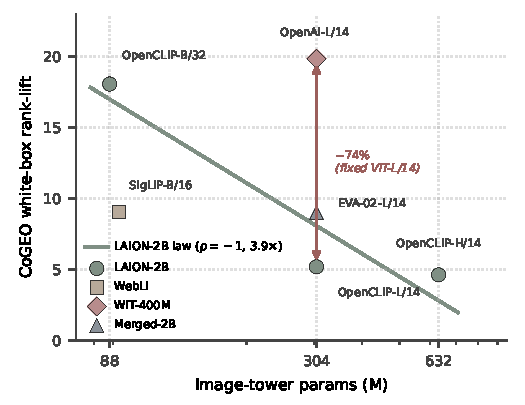
\includegraphics[width=\columnwidth]{figures/fig_capacity_scaling.pdf}
\caption{Retriever capacity compresses the manipulable band. CoGEO white-box mean rank-lift versus image-tower parameter count (log scale, $\eps=16/255$, $224\times224$): within the corpus-controlled LAION-2B family the band contracts monotonically with capacity ($18.07\to5.18\to4.61$, Spearman $\rho=-1.0$, $\approx3.9\times$); a larger or cleaner pretraining corpus compresses it further at fixed capacity ($-74\%$ from OpenAI WIT-400M to LAION-2B at ViT-L/14). The all-six correlation is a non-significant $\rho=-0.64$.}
\label{fig:extval}
\end{figure}

\paragraph{External validity beyond ESCI/OpenAI} The same four-method ordering is preserved on Food-101 (Fig.~\ref{fig:results}f), so the ceiling and ordering above are properties of the attack family rather than artifacts of the ESCI/OpenAI pairing.

\subsection{The transfer axis: significant but bounded held-out rank-lift}
\label{sec:analysis:transfer}

AE-CoGEO is the first query-free, anchor-decoupled cross-encoder probe whose role is to \emph{measure} this transfer axis as a calibrated instrument, not to mount a leaderboard or SOTA attack. One perturbation optimized against the four-encoder source consensus is scored, without re-attack, on four held-out encoders absent from the source set, against a single-encoder CoGEO reference arm (optimized against OpenAI ViT-L/14 alone) transferred to the same encoders. The only difference between arms is the source set ($n=498$ paired ESCI pairs, $\eps=16/255$), isolating the transfer mechanism (\S\ref{sec:method:aecogeo}).

\begin{table}[htbp]
\centering
\caption{Held-out-encoder transfer rank-lift (mean positions gained, $n = 498$, $\eps = 16/255$). The single-encoder arm transfers a CoGEO perturbation optimized against OpenAI ViT-L/14 alone; the AE-CoGEO arm transfers one optimized against the four-encoder source consensus (\S\ref{sec:method:aecogeo}); no held-out encoder appears in the source set. $p$: one-sided paired Wilcoxon of AE-CoGEO over the single-encoder baseline. $^{\dagger}$LAION-2B-pretrained.}
\label{tab:transfer}
\small
\setlength{\tabcolsep}{4pt}
\begin{tabular}{lrrr}
\toprule
Held-out encoder & Single-enc & AE-CoGEO & $p$ \\
\midrule
OpenCLIP-L/14$^{\dagger}$ & 1.04 & \textbf{3.29} & $7 \times 10^{-5}$ \\
OpenCLIP-H/14$^{\dagger}$ & 3.63 & \textbf{5.85} & $< 10^{-3}$ \\
OpenCLIP-B/32$^{\dagger}$ & 7.28 & \textbf{8.60} & $0.016$ \\
SigLIP ViT-B/16           & 3.07 & \textbf{4.80} & $1.3 \times 10^{-3}$ \\
\midrule
\multicolumn{4}{@{}l}{\footnotesize Strongest-source white-box: $\mathbf{18.47}$ (transfer ceiling)}\\
\bottomrule
\end{tabular}
\end{table}

\paragraph{Consensus transfer is real and statistically significant} The consensus lifts mean held-out rank-lift over the single-encoder baseline on all four unseen encoders, each gain significant at the per-comparison level (one-sided paired Wilcoxon, $p\in[7\times10^{-5},\,0.016]$; Table~\ref{tab:transfer}, Fig.~\ref{fig:results}c). A residual threat thus exists: an attacker ensembling public CLIP encoders measurably moves a retriever it never optimized against.

\paragraph{The transfer threat stays far below the white-box ceiling, across paradigms} The same source-consensus perturbation evaluated white-box on its strongest source encoder reaches the transfer ceiling of $18.47$ (Table~\ref{tab:transfer}), two-to-six times the transferred $3.3$--$8.6$. Scored without re-attack on a fused-encoder BLIP image--text reranker~\cite{li2022blip} that shares no encoder or objective with the source set ($n=500$), it reaches only $7.52$, still inside the held-out band (Fig.~\ref{fig:bounded}a): the deflation of \S\ref{sec:experiments} survives the strongest transfer attack \emph{and} a change of retrieval paradigm, and the training-free detector flags it (AUROC $0.990$).

\paragraph{Consensus transfer scales monotonically with the source-encoder count} Growing the source set from one to four public CLIP encoders raises the pooled held-out transfer monotonically ($3.76 \to 5.64$, Spearman $\rho = 1.0$; Fig.~\ref{fig:results}a), so AE-CoGEO is a genuine ensemble-transfer instrument with a measurable scaling law.

\subsection{Anchor-source robustness}
\label{sec:analysis:anchor}

\begin{figure}[tb]
\centering
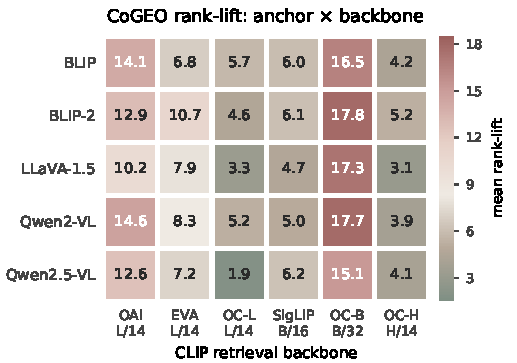
\includegraphics[width=0.92\columnwidth]{figures/fig_anchor_heatmap.pdf}
\caption{CoGEO mean rank-lift across $5$ VLM caption anchors (rows) $\times$ $6$ CLIP backbones (columns) on the $491$-ASIN ESCI manifest ($\eps=16/255$): OAI~L/14, EVA (EVA-02 L/14), OC-L (OpenCLIP L/14), SigLIP (B/16), OC-B (OpenCLIP B/32), OC-H (OpenCLIP H/14). Column means span $4.1$--$16.9$ but row means only $7.7$--$9.6$: the retriever, not the anchor captioner, explains the bulk of the spread---the signature of an anchor-decoupled protocol.}
\label{fig:anchorbb}
\end{figure}

Because the protocol requires only that the anchor be a function of $x_p$, we re-run CoGEO against the same six retrievers with five VLM captioners, giving the $5 \times 6$ rank-lift matrix of Fig.~\ref{fig:anchorbb}. Two facts hold: the retriever dominates the anchor (per-backbone column means span $4.1$--$16.9$, versus only $7.7$--$9.6$ across the five anchor captioners), and no captioner is uniformly best (within-column gap under $5$ positions). Both confirm \eqref{eq:invariant}: any function of $x_p$ alone is an admissible anchor, so the protocol surfaces an encoder-side property rather than a captioner artifact.

\subsection{Bounded under stress: transfer, defense, and scale-up}
\label{sec:analysis:summary}

The remaining robustness, transfer, and defense experiments are consolidated into one display, Figure~\ref{fig:bounded} (full per-pair data and per-experiment construction in the released artifact). Three messages emerge.

\paragraph{The white-box rank-lift is a genuine ceiling} Every out-of-source transfer probe --- a four-encoder AE-CoGEO consensus, a BLIP fused-encoder reranker, a BLIP-2 Q-Former, and a late-interaction MaxSim matcher --- stays far below it (Fig.~\ref{fig:bounded}a), so the deflation survives a change of encoder, of retrieval paradigm, and of matching mechanism. A fifth, diffusion-prior attack family lands mid-pack ($13.18$, below CoGEO's $15.60$ on the matched $n{=}500$ five-family panel; Table~\ref{tab:statsextra}), so CoGEO holds the top point estimate across five families --- though their $95\%$ CIs overlap and ranks $2$--$4$ are sample-dependent (Co-Attack $12.82$ vs $5.77$ at $560$ pairs); the per-pair distributions are strongly right-skewed for all five (Fig.~\ref{fig:distribution}).

\paragraph{The bounded operator is defender-containable, and heterogeneity is not an exploitable handle} A training-free Laplacian detector flags all four families and the AE-CoGEO transfer perturbation at AUROC $\geq0.99$, generalizing across families and to a held-out domain, degrading only as the budget shrinks (Table~\ref{tab:statsextra}); small-budget input purification removes most of the residual lift (further reduced under cohort-aware oracle allocation), and even a matched adaptive attacker stays far below the ceiling (Fig.~\ref{fig:bounded}b). A cohort-adaptive-budget (CAB) attacker redistributing a matched mean budget toward cheaper-to-move cohorts \emph{under-performs} a uniform budget ($13.0$ vs $15.6$), so heterogeneity is a diagnostic, not a handle; no tested budget is both potent and detector-evasive.

\paragraph{The findings are not small-sample artifacts} Rebuilding a label-balanced ESCI sample three times larger ($1{,}430$ pairs) sharpens the per-cohort gradient and the mean-shift, not per-pair directional dominance (Fig.~\ref{fig:bounded}c). Across all four families at this scale the mean rank-lift ordering is CoGEO $41.26 >$ Co-Attack $34.05 \approx$ PGD-bare $33.38 >$ AdvCLIP $26.16$: CoGEO has the highest mean, with Co-Attack and PGD-bare near-tied at ranks $2$--$3$. The CoGEO$-$PGD-bare lead is $+7.89$ (bootstrap 95\% CI $[2.0,13.6]$, excluding zero) yet the paired directional Wilcoxon stays non-significant ($p{=}0.78$), so the mean advantage is tail-driven; both anchor attacks nonetheless rise strictly ($E\!<\!S\!<\!C\!<\!I$), resolving rather than reproducing the small-sample $560$-pair Complement-peak ordering ($E\!<\!S\!<\!I\!<\!C$, Table~\ref{tab:cohort}), the Exact reversal vanishing. Two directional controls reinforce this: Gaussian noise at the same budget is stealthier than every attack (SSIM $0.854$) yet yields $\approx0$ rank-lift, and the same attack scored at the larger $800^2$ input is more stealthy (SSIM $\geq0.98$) but loses essentially all lift, making resolution a third trade-off axis (C3; both shown in Fig.~\ref{fig:results}e).

\begin{figure}[t]
\centering
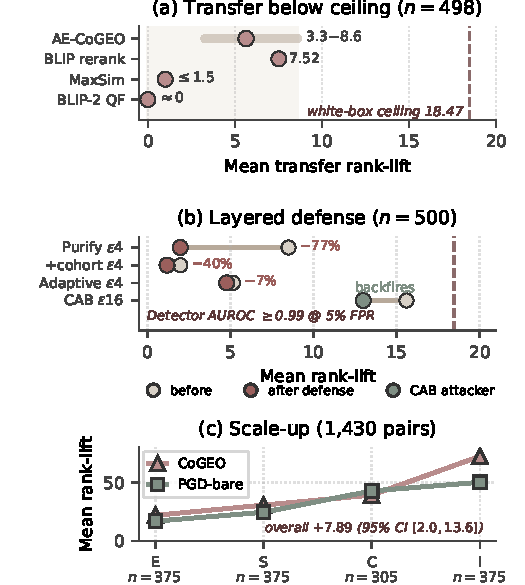
\includegraphics[width=\columnwidth]{figures/fig_bounded_defense.pdf}
\caption{Consolidated robustness, transfer, and defense evidence (rank-lift vs.\ the $18.47$ white-box ceiling; panel (c) is an independent $1{,}430$-pair scale-up with its own axis). \textbf{(a)} Out-of-source transfer: the AE-CoGEO four-encoder consensus ($3.3$--$8.6$), a BLIP fused-encoder reranker ($7.52$), a late-interaction MaxSim probe ($\leq1.5$), and a BLIP-2 Q-Former ($\approx0$) all sit far below the ceiling. \textbf{(b)} Layered defense at $\eps{=}4/255$ (before~$\to$~after): input purification ($8.50\to1.98$, $-77\%$), cohort-aware oracle ($-40\%$ further), and a matched adaptive attacker ($5.15\to4.77$); at $\eps{=}16/255$ a cohort-adaptive-budget attacker under-performs uniform ($13.0$ vs $15.6$) and a training-free detector flags every family at AUROC $\geq0.99$. \textbf{(c)} The $3\times$ scale-up sharpens the per-cohort gradient into a strictly monotone $E\!<\!S\!<\!C\!<\!I$ for both load-bearing attacks (CoGEO$-$PGD $+7.89$, 95\% CI $[2.0,13.6]$). Values match \S\ref{sec:analysis:summary}.}
\label{fig:bounded}
\end{figure}

\begin{table}[t]
\centering
\caption{Two further checks (OpenAI ViT-L/14, $n{=}500$). \emph{Top}: per-pair rank-lift for five white-box families at $\eps{=}16/255$; all are right-skewed (median $\approx1$) with CoGEO the top point estimate (overlapping CIs). \emph{Bottom}: training-free Laplacian-detector AUROC by budget, $\geq0.99$ at $\eps{=}16/255$ and degrading only as the budget shrinks.}
\label{tab:statsextra}
\footnotesize
\setlength{\tabcolsep}{4.2pt}
\begin{tabular}{@{}lrccrr@{}}
\toprule
\multicolumn{6}{@{}l}{\textbf{Five attack families (white-box), per-pair rank-lift}}\\
Family & Mean & 95\% CI & Med. & \%\,$\le0$ & Max\\
\midrule
\textbf{CoGEO} & \textbf{15.60} & [10.9, 20.3] & 1.0 & 47.0 & 354\\
PGD-bare & 13.58 & [8.3, 18.8] & 1.0 & 48.2 & 390\\
Diffusion-prior & 13.18 & [8.5, 17.9] & 1.0 & 48.8 & 388\\
Co-Attack & 12.82 & [8.2, 17.5] & 1.0 & 48.0 & 348\\
AdvCLIP & 5.06 & [1.8, 8.4] & 0.0 & 63.4 & 281\\
\midrule
\multicolumn{6}{@{}l}{\textbf{Training-free detector AUROC by budget}}\\
$\eps{=}16/255$ & \multicolumn{2}{l}{0.99--1.00} & \multicolumn{3}{l@{}}{$\eps{=}8/255$:\ 0.957--0.970}\\
$\eps{=}4/255$ & \multicolumn{2}{l}{0.852--0.889} & \multicolumn{3}{l@{}}{Food-101:\ 1.00}\\
\bottomrule
\end{tabular}
\end{table}

\begin{figure}[t]
\centering
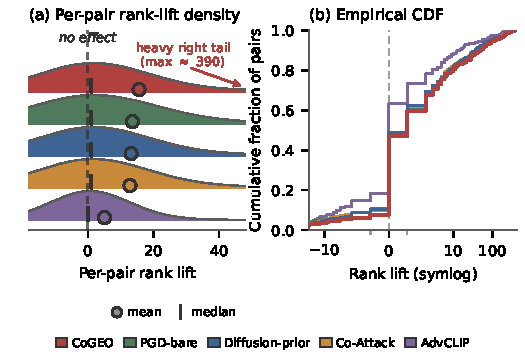
\includegraphics[width=\columnwidth]{figures/fig_distribution}
\caption{Per-pair rank-lift distribution for the five white-box attack families (OpenAI ViT-L/14, $n{=}500$ each, $\eps{=}16/255$). \textbf{(a)} Ridgeline densities: every family is strongly right-skewed---the typical pair barely moves (median $\approx1$; dashed ``no effect'' line) while a heavy right tail (up to $\approx390$) lifts the mean (open circles). \textbf{(b)} Empirical CDF on a symlog axis: the lower/further-right a curve, the heavier its tail; CoGEO is heaviest, AdvCLIP lightest, with $\geq47\%$ of pairs unaffected ($\le0$) for every family. The headline mean thus summarises a sparse, skewed effect, not a uniform shift.}
\label{fig:distribution}
\end{figure}
